\section{Operation controls, perturbations and the changed account}\label{sec:controls}
\subsection{What the operation comparison isolates}
The fixed operation study reuses exactly the same 48 aligned random-order histories of length 128, with width 12 and $H=2$. LOSSLESS performs no projection; ROUND\_ONLY rounds but has no finite code limit; CLIP\_ONLY continuously clips to $[-H,H-\Delta]$ without rounding. ROUND\_CLIP is \eqref{eq:quantizer}. SYMMETRIC\_ENDPOINT changes its code interval to $[-\upsilon,\upsilon]$, retaining the step but removing one code.

PAIR\_CLIP sums two events inside an evaluator-declared pair, then applies the original quantizer. It requires grouping/buffering unavailable to the primary autonomous event encoder and changes intermediate availability. FINAL\_CLIP projects the lossless sum once, at readout; its prefix snapshots do not feed back into future updates. CONJUGATED\_Q implements \eqref{eq:conjugacy}. These are mechanism controls, not equal-access online competitors or equal-bit-capacity implementations. Continuous values and unbounded integer codes must not be described as $b$-bit storage.

All fifteen basis/operation endpoints are in Appendix~\ref{app:data}. Directional LOSSLESS and ROUND\_ONLY both give 26 correct, three abstentions and 19 covered wrong answers out of 48. CLIP\_ONLY and ROUND\_CLIP give 48 correct, with minimum signed margins $.0539047886$ and $.0539720997$. The symmetric endpoint also gives 48 correct. Thus repeated saturation is responsible for this subset effect; rounding and endpoint asymmetry are not necessary for that particular positive quarter-lag result.

PAIR\_CLIP also gives 48 correct, with smaller minimum signed margin $.0127790302$, despite its different cadence. FINAL\_CLIP gives 48 abstentions. The independently clipped Fourier variants abstain on all 48 for every clipping operation. Fourier LOSSLESS and ROUND\_ONLY reproduce 26/3/19. CONJUGATED\_Q returns 48 correct and the same directional margins within the recorded arithmetic tolerance. These controls isolate the operator, not an advantage from renaming coordinates.

\subsection{All fixed perturbation classes}
The sixteen cells retain the same 48 order sequences. They change one factor at a time: common phases $1/16,1/8,1/4,3/8$; independent per-pair common phases; lag $1/8$ or $3/8$; common amplitudes $1/4$ or $2$; upper-only or lower-only amplitude reduction to $1/2$; bounded onset jitter; numerical range $H=1$ or $4$; or symmetric endpoints. The baseline is the remaining cell. Increasing $H$ at fixed bits also changes $\Delta$, so these are not range-only tests at fixed resolution.

The saved nuisance generator was PCG64 with SeedSequence parameters [old root,10,cell ID,old trial]; no new random orders were drawn. Jitter was uniform in $[-1/64,1/64]$, with U then L draws and a common integer offset two to keep onsets nonnegative. Actual order did not reverse in that cell. The current manuscript reads those outcomes; it does not regenerate draws.

Common phases preserve the directional signs for this subset but change margins and states. Independent pair phases give only 22/48 correct, all covered, versus Fourier 24/48. Lag $3/8$ yields directional 39 correct and nine wrong, Fourier 31 correct, one abstention and 16 wrong. Upper-half amplitude gives directional 45 correct/three wrong; lower-half gives 39/nine. The eighth-lag cell gives 48 covered wrong directional answers and 48 Fourier abstentions, as explained by Theorem~\ref{thm:eighth}. The jitter cell gives directional 48 correct and Fourier 41 correct/seven abstentions. The complete table includes the successful amplitude, range and endpoint cells; none removes the failed domains.

There are 768 perturbed histories and 12,288 reported basis/prefix records. Timestamps correctly identify every recorded actual final pair, receiving the same descriptors. Those records reuse histories and are not independent timestamp experiments or a fresh speed comparison. Prefix checkpoints are $1,2,4,8,16,32,64,128$; complete intermediate counts, saturation diagnostics and selected failure traces remain in the data supplement.

\begin{figure}[p]
\centering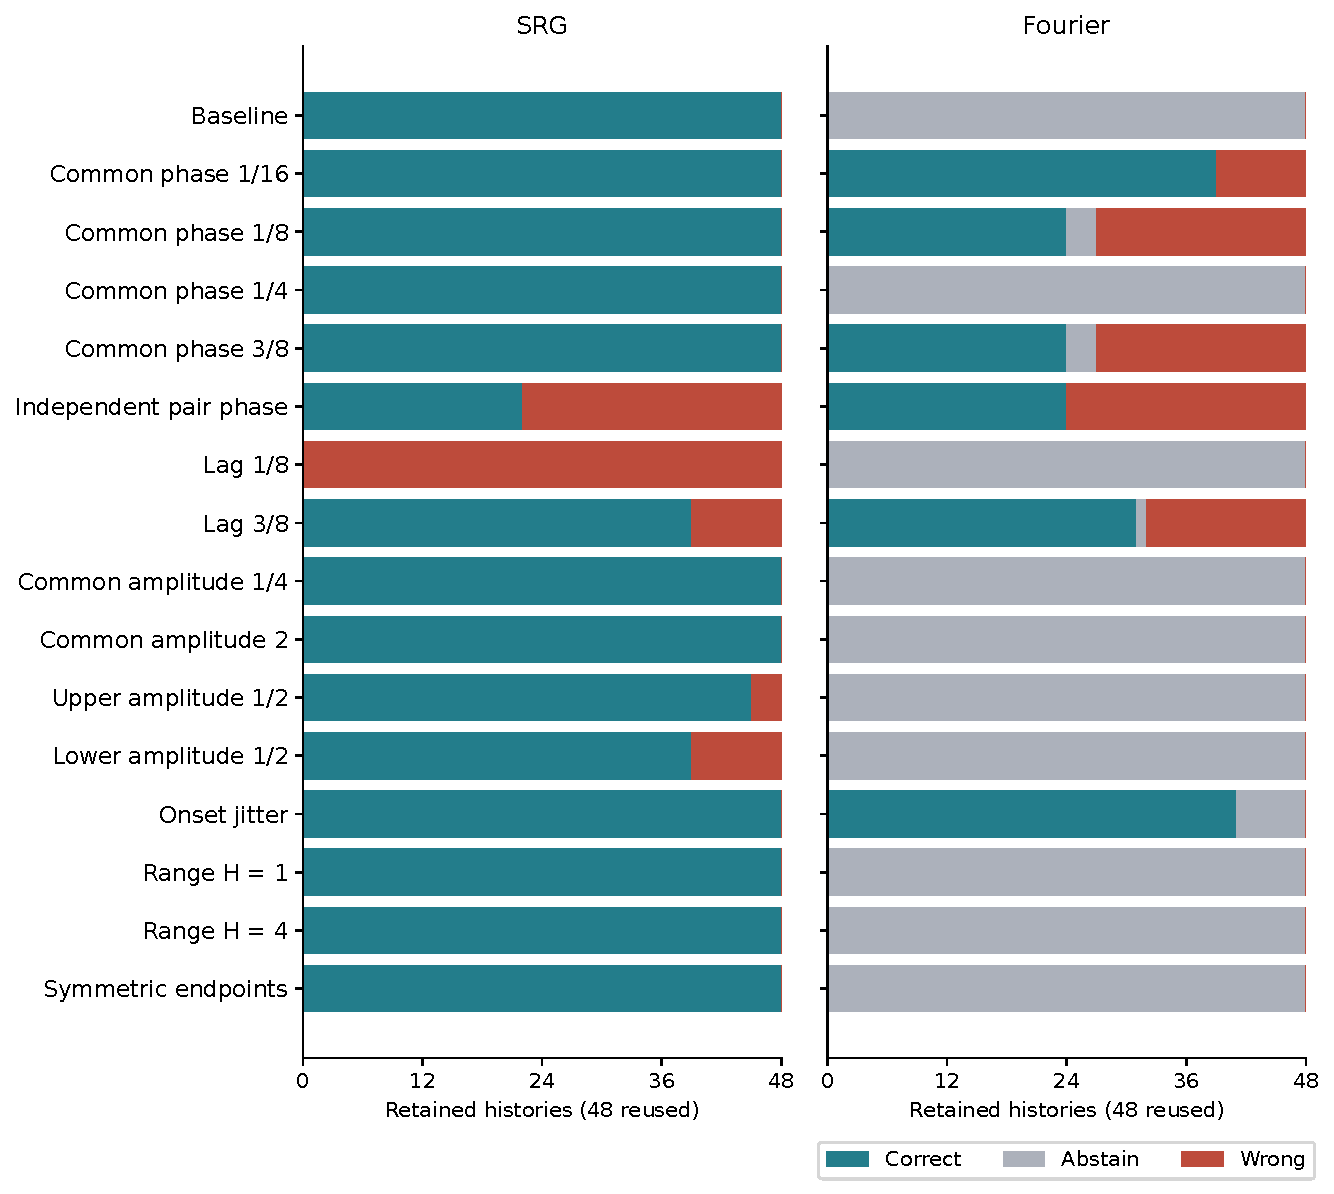
\includegraphics[width=\linewidth]{figures/fig06_controls.pdf}
\caption{All sixteen retained perturbation cells at length 128, with the same 48 order sequences reused in every cell and both bases. Correct, abstaining and covered wrong outcomes are separated. These empirical cells do not establish unrestricted phase, amplitude or history robustness.}
\label{fig:controls}
\end{figure}

\subsection{Projection is a numerical increment, not physical dissipation}
\begin{proposition}[Quadratic account under projection]\label{prop:projection}
For any directional state $x$, event increment $v$ and numerical map $Q$, let $z=x+v$, $x'=Qz$. Then
\begin{equation}\label{eq:projection}
 \E(x')-\E(x)=x\cdot v+\tfrac12\norm v^2
              +\tfrac12\bigl(\norm{Qz}^2-\norm z^2\bigr).
\end{equation}
The mean can be changed independently without affecting the harmonic decision, but remains part of the stored state and this account. In moment coordinates the corresponding metric is $\E(\Tp y)$.
\end{proposition}
\begin{proof}
Add and subtract $\norm{x+v}^2/2$, then expand its difference from $\norm x^2/2$. Coordinatewise quantization updates the mean without mixing it into the four harmonic coordinates; the decision \eqref{eq:storage} contains no mean. This proves decision independence, not permission to omit the mean from storage. Substitution $x=\Tp y$ gives metric matrix $\Tp^{\mathrm T}\Tp/2$ in moment variables.
\end{proof}
The final bracket is an additional numerical projection term. Pure axis clipping toward an interval containing zero cannot increase any absolute coordinate, so its Euclidean contribution is nonpositive; rounding can increase it. Independent Fourier-axis clipping is not Euclidean projection in the $\Tp^{\mathrm T}\Tp$ metric and need not share that argument.

At length 128 the clipped mean is at most $2-\Delta$ instead of 128, replacing the lossless mean account 8192 by approximately two. This is a different state. The projection term is not an implementation of C1 source work, native heat, emitted energy, physical dissipation or a conserved physical quantity.

Diagnostics distinguish overflow of a \emph{rounded code} from a direct unrounded value outside the interval. A small direct residual can round to an allowed boundary and produce no overflow count. CLIP\_ONLY retains the original rounded-trigger diagnostic separately from actual continuous clipping. Traces also record rounding changes, signed and absolute lost increments and projection-account changes. These belong to the evaluator and never enter the decoder.

The single mechanism evaluation took $56.843$ s, with peak working set 111,869,952 bytes and peak pagefile use 127,045,632 bytes. It is not a new cost contest. Its initial precheck failed at Python's integer-string serialization limit; only presentation of enormous rational bounds was changed to compact outward bounds, preserving proof arithmetic and scoring. The accepted record retains that failure, fourteen successful pre-run groups, eight saved-result audit groups and a separate rational eighth-lag certificate. These historical counts are not new manuscript validations.
